\subsection{Incidencias del Proyecto}
En esta sección del TFG, se aborda uno de los aspectos más importantes del desarrollo 
de un proyecto de Machine Learning: los problemas y desafíos que pueden surgir durante 
el proceso. Es común que se presenten dificultades que pueden afectar tanto la precisión 
como la eficiencia del modelo. Estos problemas pueden ser causados por una variedad 
de factores a continuación se describen algunos de los inconvenientes que se presentaron
durante el desarrollo del proyecto.

\subsubsection{Problemas con la normalización de los datos}
La normalización de los datos de entrada es un paso crítico para garantizar que el 
modelo pueda aprender de manera efectiva y generar predicciones precisas. En el caso 
específico de los grafos, el estado de un nodo puede almacenar diferentes tipos de datos, 
como números, referencias a otros nodos, etc, lo que puede generar problemas a la hora 
de la normalización. Otro lugar done también surgen problemas de normalización es en los 
datos de las aristas, que representan las conexiones entre nodos. Al respresentar un 
nodo como una lista de características, estas diferentes caracteristicas de pueden 
requerir de diferentes técnicas de normalización.\medskip

La soluación que se ha adoptado en este proyecto es la de normalizar los datos de
cada entrada de manera independiente. De esta manera, se evitan problemas de colision 
entre los diferentes nodos y aristas de un mismo grafo. Esta solución, sin embargo,
trae problemas de escalabilidad ya que cada vez que se implementa y/o añade una nueva
característica al modelo, es necesario modificar el código de normalización de los datos.\medskip

En un futuro, se podría implementar una solución más escalable, que permita definir
un conjunto de tipos de características con sus respectivas técnicas de normalización.
De este modo, se podría añadir nuevas características al modelo sin necesidad de
modificar el código de normalización. Además, tambien daria la posibilidad de
poder en una fase de testeo, probar diferentes técnicas de normalización para
cada tipo de característica y elegir la que mejor se adapte al modelo.

\subsubsection{Problemas con el hardware de entrenamiento}
La falta de hardware adecuado para el entrenamiento y testeo es un problema común 
que puede afectar la eficiencia y la precisión del modelo. El entrenamiento de modelos 
de Machine Learning a menudo requiere una gran cantidad de recursos computacionales, 
como procesadores, memoria RAM y capacidad de almacenamiento. Además, los modelos 
pueden requerir GPUs (unidades de procesamiento gráfico) especializadas para acelerar 
el proceso de entrenamiento.\medskip

La falta de hardware adecuado puede limitar la cantidad de datos que se pueden usar 
para entrenar el modelo, la complejidad del modelo que se puede entrenar y la 
velocidad a la que se puede realizar el entrenamiento. Esto puede resultar en 
modelos que no sean lo suficientemente precisos o que no se puedan entrenar en 
un tiempo razonable. En el caso de este proyecto, se ha contado con un pequeño
servidor que disponia de una CPU y 4GB de RAM, lo que ha limitado el tamaño de los
grafos que se han podido usar para el entrenamiento. Además, el entrenamiento de
los modelos y la búsqueda de hiperparámetros ha sido un proceso lento, ya que
no se ha contado con una GPU para acelerar el proceso.\medskip

En un futuro, se podría implementar una solución que permita entrenar los modelos
utilizando una o varias GPUs. Esto permitiría entrenar modelos más complejos
con un mayor número de parámetros y con un mayor número de datos de entrenamiento.

\subsubsection{Problemas de rendimiento}
Python es un lenguaje de programación interpretado, lo que significa que el código
se ejecuta línea por línea, en lugar de compilarlo en un programa ejecutable. Esto
hace que sea extremadamente lento en comparación con otros lenguajes de programación
como es el caso de C o C++. Es por ello que durante el desarrollo del proyecto, se
ha tenido que realizar varias tareas de profiling para identificar las partes del
código que más tiempo de ejecución consumían y optimizarlas.\medskip

Para ello se ha utilizado la librería \textit{cProfile} de Python, que permite
realizar un análisis de rendimiento del código. Esta librería genera un informe
con el número de llamadas y el tiempo de ejecución de cada función del código.
De este modo, se puede identificar las funciones que más tiempo de ejecución
consumen y optimizarlas.\medskip

\begin{figure}
    \centering
    \begin{minipage}{0.47\textwidth}
        \centering
        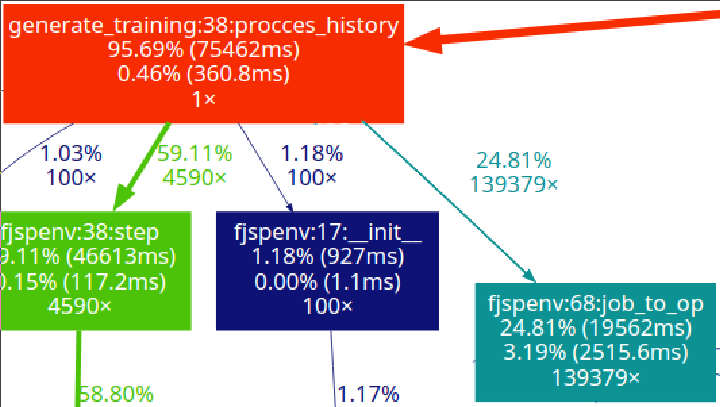
\includegraphics[width=0.85\textwidth]{before-fix.png} 
        \caption{Environment no optimizado}
    \end{minipage}\hfill
    \begin{minipage}{0.47\textwidth}
        \centering
        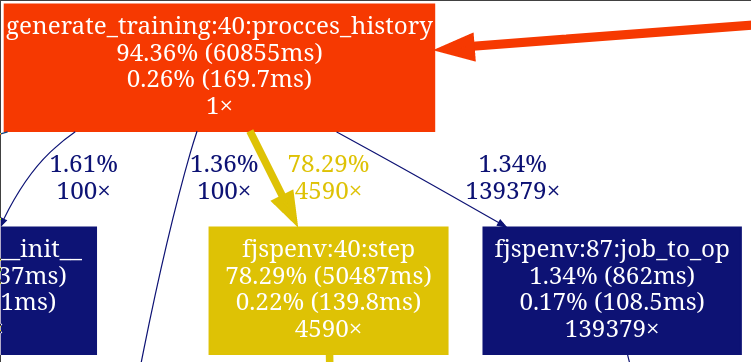
\includegraphics[width=1\textwidth]{after-fix.png}
        \caption{Environment optimizado}
        \label{fig:after-fix}
    \end{minipage}
\end{figure}

En este caso en concreto en el que se puede ver la diferencia de rendimiento
entre el código no optimizado y el código optimizado, debido a que la función
\textit{job\_to\_op} del environmente que se encarga de transformar un trabajo
en una operación para poder actulizar el estado del grafo, se ejecuta un gran
número de veces durante el entrenamiento. Por ello, se ha optimizado el código
de esta función para que sea más eficiente utilizando una utlidad de Python
llamada \textit{functools.lru\_cache}, que permite cachear los resultados de
una función para evitar tener que ejecutarla varias veces con los mismos
parámetros.\medskip

Como se puede ver en la figure \ref{fig:after-fix}, el tiempo de ejecución
se ha reducido un 24\% del tiempo total de ejecución del código. Si quisieramos
optimizar aún más el código, se podría implementar algunas de las funciones
del environment en C++ y luego importar el módulo en Python, aunque esto
requeriria un mayor esfuerzo de desarrollo. 